\chapter{Evaluation of connect four bots}
\label{ch:connect_four_eval}

The previous chapter discussed the two \gls{dqn} agents and the Rainbow agent that were implemented for this project.
Section \ref{sec:marl-games_opponent} discussed how the learned policy of the agents would be used as a computer-opponent in the connect four game and thus should be subjectively pleasing to play against rather than objectively good according to a specific metric.
This chapter will aim to evaluate the policies obtained throughout various experiments with these \gls{rl} agents.

%------------------------------------

\section{Objective evaluation of the emerged policies}
\label{sec:connect_four_eval-metrics}

As discussed in section \ref{sec:marl-games_opponent}, objective evaluation metrics of the \gls{rl} agents have small value in this feasibility study.
An agent that wins all the time is objectively very good, but since connect four is a solved game and a perfect policy for the agent playing as player 1 exists, the objectively best agent would be one that is unbeatable, making it rather useless as a computer-controlled opponent in a video game.
Likewise, it could be argued that an agent who wins in very few steps is objectively better than one that wins in many steps.
However, when letting an \gls{rl} agent train against a random agent, the \gls{rl} agent simply learns to stack coins in a singular column.
This same behaviour is also present when doing self-play and only providing rewards for a win, loss or a tie.
This is the case for both \gls{dqn} agents as well as for the rainbow agent, although some agents seem to learn to block some winning moves as well, yet stick to the stacking strategy.
This behaviour is statistically sound when playing against a random agent, as the random agent would only block the vertical win 3 out of 7 times, resulting in a win in four moves 4 out of 7 times for the \gls{rl} agent.
However, in self-play, this behaviour is not statically sound and it is very likely that given more training iterations, these policies would diverge from the stacking behaviour into a better policy, as some signs of blocking behaviour emerged after half an hour of CUDA training.
However, the metric based on wins and favouring shorter average game length would score this stacking policy highly, but it is almost worthless in human play.
An example of this bad policy is shown in figure \ref{fig:stacking_behaviour}.

\begin{figure}[ht]
    \centering
    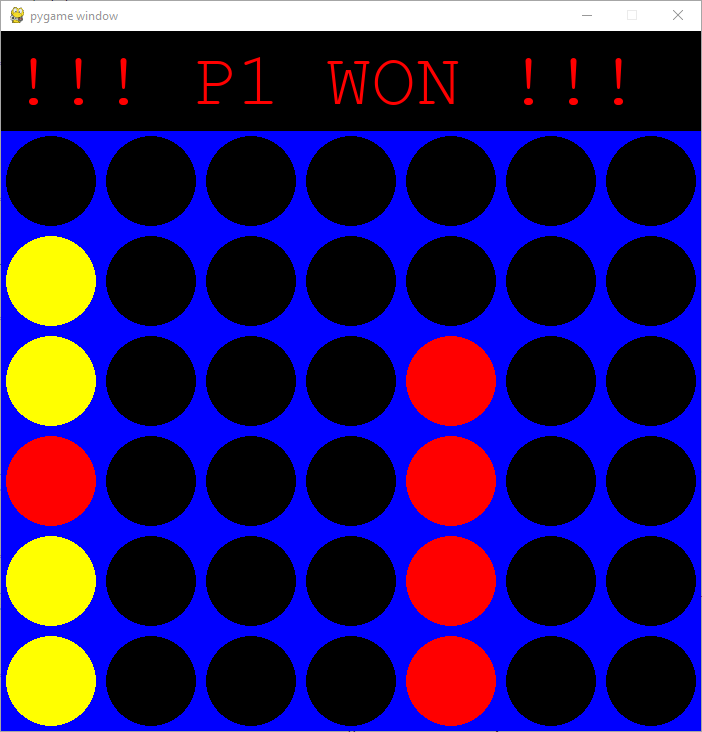
\includegraphics[width=0.4\linewidth]{images/naive_policy.png}
    \captionsetup{width=0.9\linewidth}
    \captionsetup{justification=centering}
    \caption{The MLP DQN agents having both learned stacking policies through self-play, with the agent playing as player 1 having some blocking behaviour as well. This policy would score good on some objective measures but is near worthless as a computer-opponent.}
    \label{fig:stacking_behaviour}
\end{figure}

When optimising for a metric where longer games are favoured, with the idea that playing a long game requires the blocking of winning moves, a similar trend occurs where a good scoring policy is worthless in human play.
Indeed, a policy which gets draws through self-play every time has maximal game length and maximal summed scores since both agents are positively rewarded for a draw.
This policy can be achieved by rewarding the agents of either proposed algorithm for making moves and coming to ties.
Since the maximum reward is obtained when getting a tie, the agents learn a policy that goes for ties.
This involves deliberately ignoring win potentials and learning to play as a team with the other agent in self-play rather than playing against it.
Thus, the resulting algorithm is again useless in human play. 

One interesting objective evaluation that can be made is the performance of an agent playing as player 1 vs it playing as player 2.
\Citet{connectfour_rl} concluded for their connect four agents that an agent playing as player 1 in self-play is far more likely to win over an agent playing as player 2.
They hinted that this could be due to the solved nature of the connect four game where an optimal policy exists for player 1 to ensure a win every time.
When looking at the training results of a Rainbow agent against a varying depth mini-max agent given in Table \ref{tab:minimax_learning} it becomes clear when playing as player 1, the agent does indeed learn faster and the best policy is indeed better.
However, the found policy is far from the optimal policy that results in a win each time, as will become clear when looking at the win rate against even a simple random agent.
Thus, we suspect the difference between the performance of playing as player 1 or player 2 originates from the fact that player 2 always has one coin less on the board when doing his move.

Another interesting objective metric is looking at the win rate of the trained \gls{rl} agent against a random agent.
This can give some insight into how good a given policy is since a random agent should be relatively simple to beat.
Figure \ref{fig:win_rate_random} shows the win rate against the random opponent for the best-found policy of all three \gls{rl} agents.
This further shows that the \gls{rl} agent playing as agent 1 is indeed better than the best-found policy learned when playing as player 2.
It also becomes clear that the Rainbow policy seems to outperform the \gls{dqn} based policies.
The difference between the \gls{mlp} based \gls{dqn} and \gls{cnn} based \gls{dqn} is negligible.
This corresponds with the findings surrounding the human-play behaviour of these algorithms, although there the Rainbow policy is far better than the \gls{dqn} policies.

\begin{figure}[ht]
    \centering
    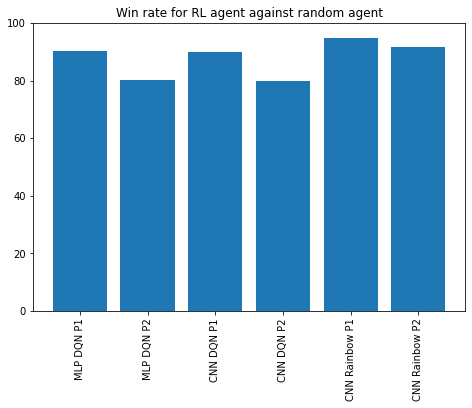
\includegraphics[width=0.7\linewidth]{images/rl_vs_random.png}
    \captionsetup{width=0.9\linewidth}
    \captionsetup{justification=centering}
    \caption{Win rate of the best found \gls{rl} policy against a random agent. All three of the discussed policies are used once as player 1 and once as player 2. The results are averaged over 1000 games.}
    \label{fig:win_rate_random}
\end{figure}




%------------------------------------

\section{Usability of deep Q-network policy as connect four bot}
\label{sec:connect_four_eval-dqn_vs_human}

The two \gls{dqn} approaches, one using a \gls{mlp}-based model and one using a \gls{cnn}-based model, showed similar trends throughout all experiments when used in human-play.
When training the \gls{rl} agents through self-play and only providing a reward for wins, losses and ties, the learned policy is the stacking behaviour discussed in section \ref{sec:connect_four_eval-metrics} and shown in Figure \ref{fig:stacking_behaviour}.
This was the case for the best-found policy and final policy after training on 1 million steps in the connect four game.
This was done through 1000 epochs consisting of 1000 steps per epoch and updating the agent's policy every 64 steps.
This behaviour is near worthless in human play.
When also providing a reward for making moves, the agents learn to play together as was also already discussed in section \ref{sec:connect_four_eval-metrics}.
Since this agent assumes the other agent wouldn't go for a winning move as it also wants to prolong the game for as long as possible, the final obtained policy through a similar training procedure as before is again non-satisfactory in human play.

In an attempt to improve this behaviour, an experiment was set up inspired by a league-based approach.
Alternating in varying frequencies, one agent was frozen so that it doesn't learn whilst the other was unfrozen so that it does learn.
This was done for a decreasing amount of epochs per freezing alternation, but an increasing amount of alternations in 7 different experiments for both \gls{dqn} policies.
Each time the new experiment started both agents with the best-found policy of the previous experiment.
According to the definition given in section \ref{sec:marl-vs_single} this makes the problem a single-agent \gls{rl} problem and this reduces the non-stationary problem.
This was done for a considerable amount of training time and exact details can be found in paper notebooks 7 and 8 which are available on the GitHub repository of this project \citep{github_project}.
However, this seems to result in the agents overfitting to each other's policy rather than a more pleasing human play policy.
This can be seen by the agent's being capable of winning a lot against the frozen opponent but losing just as much when frozen itself.

No experiments on the \gls{dqn} agents were done using the reward for making a blocking move, as it was only introduced when working with Rainbow agents.
This leaves the \gls{dqn} agents with no real pleasing found policy for human play.
It is noted that if an experiment were to be done using a reward for making blocking moves, it is likely it would cause a more promising policy to emerge.

The \gls{dqn} agents likely suffer from something that is called catastrophic forgetting.
This phenomenon occurs when a model is training on new unseen data and forgetting the things it has learned in the past.
This could explain why the alternating freezing of the agents didn't yield a more pleasing human-play result since it could be possible the learned blocking techniques in previous iterations are being forgotten in new iterations.
The fact that the batch size is 1 for these \gls{dqn} agents also doesn't aid with this potential problem.
However, known issues when combining the Tianshou library's batch mechanism and multi-agent policies forced the \gls{dqn} implementations of this paper to work with a batch size of 1.
Catastrophic forgetting is a common issue with \glspl{dnn} as further explained by \citet{catastrophic_forgetting}.
The performed experiments described above can all be found in paper notebooks 4 to 8 which are available on the GitHub repository of this project \citep{github_project}.

%------------------------------------

\section{Usability of Rainbow policy as connect four bot}
\label{sec:connect_four_eval-rainbow_vs_human}

Since the Rainbow policy is known to be both more sample-efficient and better performing than \gls{dqn}, as discussed in section \ref{sec:connect_four_rl-rainbow}, even more effort was put into making a pleasing Rainbow policy for human play.
This policy doesn't suffer from the issue of having to use a batch size of 1 and uses a batch size of 64 throughout all experiments.

When using a reward for making a move as well as a reward for winning, losing and getting a tie, the learned policy is more interesting than was the case for the team playing agents with \gls{dqn}.
This is shown in Figure \ref{fig:tie} where the yellow player performs blocking moves in self-play, even though no specific reward is given for playing a blocking move.
However, when greeted with the chance to win, as was the case for getting a horizontal win in the second row from the bottom, the yellow agent doesn't seem to go for this winning move.
This is likely since it wants to prolong the game and go for a tie rather than go for a win now, as the latter yields a lower total reward.
Although not very frequent, this training procedure did result in some tie games.
Since the second player has some move blocking behaviour, it forms a somewhat interesting computer-opponent in human play, although it mostly seems to block vertical wins and almost always fails to block horizontal or vertical wins.

\begin{figure}[ht]
    \centering
    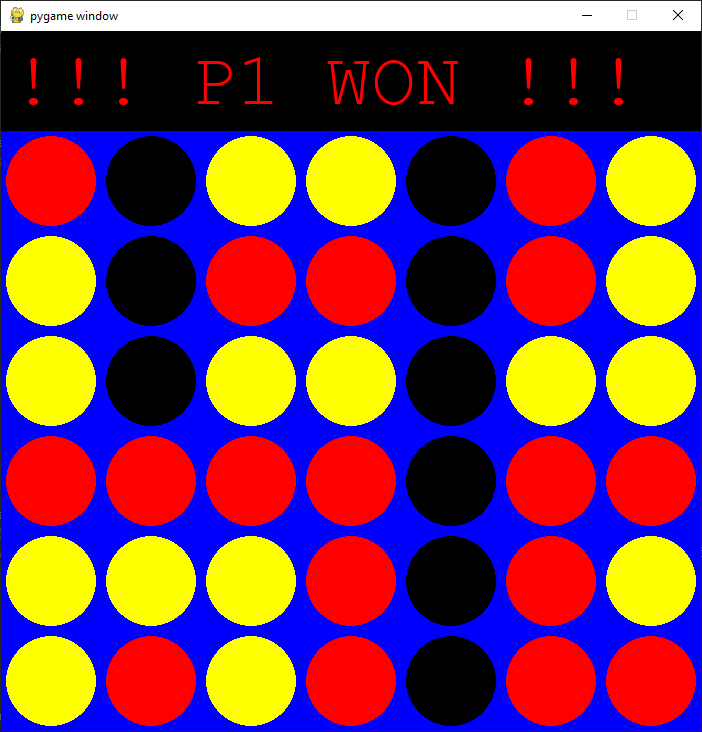
\includegraphics[width=0.4\linewidth]{images/near_tie.png}
    \captionsetup{width=0.9\linewidth}
    \captionsetup{justification=centering}
    \caption{Rainbow policy self-play in an environment where a reward is given for making a move. The policy tends to go for getting as many moves as possible. For example, the agent playing as yellow does perform win blocking moves but doesn't do moves that would result in a win when given the opportunity.}
    \label{fig:tie}
\end{figure}

Since the policy from rainbow showed some promising signs of intelligence, it was opted to help it become better by rewarding it for making a blocking move.
This reward strategy was already discussed in section \ref{sec:connect_four_rl-rewards}.
By doing so, the agent became significantly more powerful.
When playing against the best-found policy for player 1 of this training procedure, games like the one shown in Figure \ref{fig:rainbow_diagonal_win_turn_annotation} are obtained through human play.
The agent manages to block vertical and horizontal wins early on but fails to block the final diagonal winning move made by the human.
When playing against this bot multiple times, a pleasant experience can be had, but some flaws do show up.
The stacking coin strategy isn't blocked when done in the far left or right corner of the board, as is shown in Figure \ref{fig:rainbow_failed}.
It is expected that this follows from the fact that through the convectional layer, centre columns are present in multiple kernel passes whilst the edge columns are only present in one pass per row.
It is assumed that a longer training procedure would likely improve this behaviour, although it was not feasible given the computational power at hand.
Similarly, the blocking behaviour of horizontal rows works well in the early stages of the game, where the lower rows are played but when playing in the upper rows of the board, the blocking behaviour seems to disappear only to be present in very specific boards.
This is likely again caused by the fact almost all training samples contain player coins in the lower rows of the board but coins in the higher rows of the board are rather rare.
Training for a longer period could again possibly solve this issue.

\begin{figure}[ht]
    \centering
    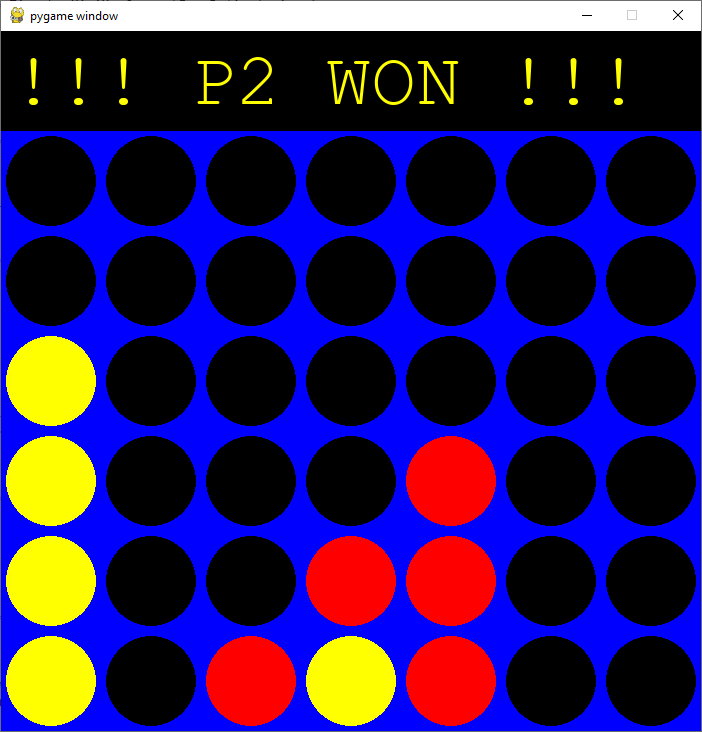
\includegraphics[width=0.7\linewidth]{images/rainbow_failed_policy.png}
    \captionsetup{width=0.9\linewidth}
    \captionsetup{justification=centering}
    \caption{Sample connect four game with the best-found rainbow policy (player 1, red) from the paper notebook 9, and a human. The best-found policy struggles in blocking winning horizontal moves placed in the far left corner or far right corner.}
    \label{fig:rainbow_failed}
\end{figure}

When using the same freezing technique as was done for the \gls{dqn} algorithms, the algorithm once again overfits to the opponent's policy and/or suffers from catastrophic forgetting.
This results in a high win rate against the frozen agent but a worse human play policy.
The performed experiments described above can all be found in paper notebooks 9 and 10 which are available on the GitHub repository of this project \citep{github_project}.

%------------------------------------

\section{Viability of varying difficulty bot performance}
\label{sec:connect_four_eval-varying_difficulty}

In an attempt to further increase the performance of the Rainbow agents, a different approach to league-based training is done.
Instead of using a frozen agent to play against, an increasing depth mini-max agent is played against.
The ideology behind this is explained in section \ref{sec:connect_four_rl-minimax_opponent}.
Since the mini-max calculations take a considerable amount of time, experimenting once as player 1 and once as player 2, took over 72 hours.
Each iteration of the mini-max opponent was trained for either 250 epochs or when an average test score of at least 10 was obtained.
The latter test score would correspond with an average combination of winning (5) and making 5 blocking moves ($5*1$), getting a tie (3) and making 7 blocking moves ($7*1$) or losing (-5) but making 15 blocking moves ($15*1$).
All of these behaviours would be pleasant human play behaviours.
The training results are given in Table \ref{tab:minimax_learning}.

However, as was discussed in section \ref{sec:marl_opponents}, league based opponents should not only increase in difficulty, but they should also not be too predictable to combat potential overfitting on the opponent's policy rather than better learning to play the game.
This behaviour was present when doing the frozen agent approach, and it was thought that the adaptation from the mini-max agent to a certain move would reduce this overfitting behaviour.
However, the final policies obtained from this experiment were not that satisfactory in human play, hinting that the same issues as was the case when freezing the opponent occurred.
Although this time it is more likely to be a type of catastrophic forgetting rather then overfitting and ideally the experiment should be redone using a decaying learning rate to try and mitigate this problem.
However, due to the lengthy computations, this was not feasible for this project.
If the experiment was redone using a decaying learning rate and potentially using other tricks to help and combat catastrophic forgetting, the author of this paper believes this approach could provide varying difficulty bots. 

\begin{table}[ht]
    \centering
    \begin{tabular}{|l|l|l|}
    \hline
    \textbf{Mini-max depth} & \textbf{Player 1 best test score} & \textbf{Player 2 best test score} \\ \hline
    1                      & 10.82 ± 0.24 in epoch 182         & 9.78 ± 1.56 in epoch 186          \\ \hline
    2                      & 10.70 ± 0.00 in epoch 45          & 10.20 ± 0.00 in epoch 217         \\ \hline
    3                      & 11.30 ± 0.00 in epoch 11          & 10.90 ± 0.00 in epoch 73          \\ \hline
    4                      & 10.48 ± 3.66 in epoch 6           & 7.10 ± 0.00 in epoch 132          \\ \hline
    5                      & 10.90 ± 0.00 in epoch 6           & 6.90 ± 0.00 in epoch 27           \\ \hline
    \end{tabular}
    \captionsetup{width=0.9\linewidth}
    \captionsetup{justification=centering}
    \caption{\label{tab:minimax_learning} Results of letting Rainbow agents play against a varying depth mini-max agent. Maximum amount of training epochs is 250 per mini-max depth and the stopping criteria is set to a test score of over 10.}
\end{table}